\documentclass[12pt]{beamer}

\usetheme{Oxygen}
\usepackage{thumbpdf}
\usepackage{wasysym}
% \usepackage{ucs}
\usepackage[utf8]{inputenc}
\usepackage{pgf,pgfarrows,pgfnodes,pgfautomata,pgfheaps,pgfshade}
\usepackage{verbatim}
\usepackage{multicol}

\pdfinfo
{
  /Title       (Taller de Desarrollo Web)
  /Creator     (TeX)
  /Author      (Sebastián Salazar Molina)
}


\title{Taller de Desarrollo Web}
\subtitle{Laravel}
\author{Sebastián Salazar Molina.}
\institute[INF - UTEM] { Unidad de Informática - Universidad Tecnológica Metropolitana }
\date{27 de Abril de 2014}

\begin{document}

\frame{\titlepage}

\section*{}
\begin{frame}
  \frametitle{Contenidos}
  \begin{multicols}{2}
    \tableofcontents[section=1,hidesubsections]
  \end{multicols}
\end{frame}

\AtBeginSection[]
{
  \frame<handout:0>
  {
    \frametitle{Contenidos}
    \begin{multicols}{2}
    \tableofcontents[currentsection,hideallsubsections]
    \end{multicols}
  }
}

\AtBeginSubsection[]
{
  \frame<handout:0>
  {
    \frametitle{Contenidos}
%     \begin{multicols}{2}
    \tableofcontents[sectionstyle=show/hide,subsectionstyle=show/shaded/hide]
%     \end{multicols}
  }
}

\newcommand<>{\highlighton}[1]{%
  \alt#2{\structure{#1}}{{#1}}
}

\newcommand{\icon}[1]{\pgfimage[height=1em]{#1}}



%%%%%%%%%%%%%%%%%%%%%%%%%%%%%%%%%%%%%%%%%
%%%%%%%%%% Content starts here %%%%%%%%%%
%%%%%%%%%%%%%%%%%%%%%%%%%%%%%%%%%%%%%%%%%



% Introducción
\section{Introducción}
\subsection{Introducción}

\begin{frame}
\frametitle{Acerca de mí.}
\begin{itemize}
 \item<2-> Sebastián Alexis Salazar Molina (@sebastian\_sm) .
 \item<3-> Ingeniero Civil en Computación (UTEM).
 \item<4-> Consultor TI en \href{http://www.experti.cl}{ExperTI} (C/C++ , PHP, Java)
 \item<5-> \href{http://sebastian.cl}{http://sebastian.cl}
\end{itemize}
\end{frame}


\begin{frame}
\frametitle{Acerca del taller.}

Este taller está pensado para personas sin conocimientos previos y es una aproximación muy básica e inicial hacia el desarrollo web, usando el framework Laravel.
\end{frame}


\begin{frame}
\frametitle{Temas}
Los temas que se trataremos son:
\begin{itemize}
 \item<1-> Herramientas.
 \item<2-> Servidores Web.
 \item<3-> HTML / CSS.
 \item<4-> JavaScript / jQuery.
 \item<5-> PHP.
 \item<6-> SQL / PostgreSQL.
 \item<7-> Laravel.
\end{itemize}
\end{frame}

\section{Herramientas}

\subsection{Computador}

\begin{frame}
 \frametitle{Computador}
 La principal herramienta del Desarrollador, es su \alert{computador}.
 \newline
 Deben adquirir un \alert{buen} computador, tenga presente que pasará más de 8 horas diarias frente a un computador.
\end{frame}


\begin{frame}
 \frametitle{Enfermedades comunes.}
 \begin{itemize}
  \item<2-> Daños a la vista.
  \item<3-> Síndrome del túnel Carpiano.
  \item<4-> Molestias en la Espalda.
  \item<5-> Problemas a la salud mental.
 \end{itemize}
\end{frame}

\subsection{Software}

\begin{frame}
 \frametitle{Software}
 El siguiente paso es disponer del software adecuado, para el propósito de nuestro trabajo. Un buen editor de texto, nos facilitará mucho el trabajo, sin embargo escoger un buen ide, nos ahorrá mucho tiempo.
 \newline
 Algunos Editores e IDEs populares
 \begin{itemize}
  \item Open Komodo
  \item Kdevelop
  \item Eclipse
  \item Sublime Text
  \item NetBeans
 \end{itemize}
\end{frame}



\section{Servidores Web}

\begin{frame}
 \frametitle{Servidores Web}
 Un servidor web, es un software que se ejecuta en un servidor, que permite realizar conexiones bidireccionales y/o unidireccionales y síncronas o asíncronas con un cliente, generando o cediendo una respuesta en cualquier lenguaje o Aplicación del lado del cliente. 
 \newline
 Generalmente se usa el protocolo HTTP para estas comunicaciones, perteneciente a la capa de aplicación del modelo OSI. El término también se emplea para referirse al ordenador que ejecuta el programa.
\end{frame}


\begin{frame}
 \frametitle{Servidores Web}
 Existen una amplia oferta de servidores web, algunos son de propósito general, otros están enfocados a correr aplicaciones en un lenguaje específico, esto es importante porque nos permitirá escoger la mejor alternativa según nuestras necesidades.
\end{frame}


\begin{frame}
 \frametitle{Servidores Web}
 \begin{itemize}
  \item Nginx ( http://nginx.org/ )
  \item Apache HTTPD ( http://httpd.apache.org/ )
  \item Internet Information Services (IIS) ( http://www.iis.net/ )
  \item Cherokee ( http://cherokee-project.com/ )
  \item Tomcat ( http://tomcat.apache.org/ )
  \item lighttpd ( http://www.lighttpd.net/ )
  \item thttpd ( http://www.acme.com/software/thttpd/ )
  \item monkeyd ( http://monkey-project.com/ )
 \end{itemize}
\end{frame}

\begin{frame}
 \frametitle{Servidores Web}
 La mayoría de los servidores web, son modulares y ofrecen características extendidas, al agregar módulos. En mi opinión, el servidor web más sencillo de usar es apache, viene en casi todas las distribuciones, y en windows existen muchos paquetes que lo tienen como parte integral de sus soluciones.
\end{frame}

\section{HTML / CSS}

\subsection{HTML}

\begin{frame}
 \frametitle{HTML}
 HTML, es la sigla para HyperText Markup Language (lenguaje de marcas de hipertexto), es un estándar que hace referencia al lenguaje de marcado para la elaboración de páginas web. Este estándar define una estructura básica y un código (denominado código HTML) para la definición de contenido de una página web, como texto, imágenes, etc. Está a cargo de la W3C.
 \newline
 El HTML se escribe en forma de ``etiquetas''. HTML permite la inclusión de script y hojas de estilo, que alteran el comportamiento de la página web.
\end{frame}

\begin{frame}
 \frametitle{Estructura}
 \begin{center}
    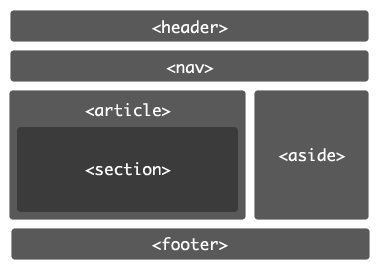
\includegraphics[scale=0.5]{img/html5structure.png}
 \end{center}
\end{frame}

\begin{frame}
 \frametitle{Estructura}
 \begin{center}
    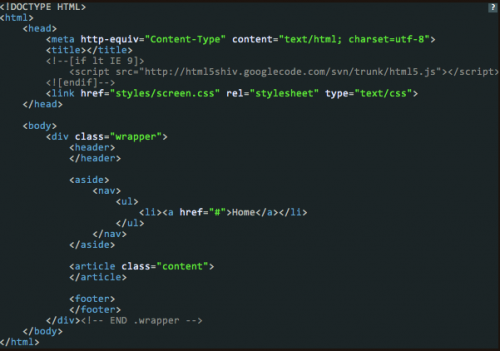
\includegraphics[scale=0.5]{img/html5code.png}
 \end{center}
\end{frame}


\begin{frame}
 \frametitle{Atributos}
 Cada etiqueta tiene atributos específicos, sin embargo, existen un conjunto de atributos comunes a todos los elementos.
 \begin{itemize}
  \item<2-> \alert{id} este atributo debe ser único en el documento y representa el identificador de la etiqueta.
  \item<3-> \alert{class} este atributo permite definir una regla CSS que la etiqueta debe cumplir.
  \item<4-> \alert{style} este atributo permite introducir reglas específico de CSS.
  \item<5-> \alert{title} El título de la etiqueta que se despliega al posar el mouse sobre el elemento.
 \end{itemize}
\end{frame}


\begin{frame}
 \frametitle{Atributos}
 Recuerde \href{http://www.w3schools.com/html/default.asp}{http://www.w3schools.com/html/default.asp} es su amigo.
\end{frame}

\subsection{CSS}

\begin{frame}
 \frametitle{CSS}
 Las Hojas de Estilo en Cascada (Cascading Style Sheets) es el lenguaje de hojas de estilo utilizado para describir el aspecto y el formato de un documento escrito en un lenguaje de marcas, esto incluye varios lenguajes basados en XML como son HTML, XHTML o SVG.
 \newline
 La ventaja es que los estilos se pueden adjuntar en un documento separado o en el mismo documento HTML. En este último caso podrían definirse estilos generales en la cabecera del documento o en cada etiqueta particular mediante el atributo ``style''.
\end{frame}

\begin{frame}
 \frametitle{CSS}
 Una hoja de estilo se compone de una lista de reglas. Cada regla o conjunto de reglas consiste en uno o más selectores y un bloque de declaración (o ``bloque de estilo'') con los estilos a aplicar para los elementos del documento que cumplan con el selector que les precede. 
 Cada bloque de estilos se define entre llaves, y está formado por una o varias declaraciones de estilo con el formato \alert{propiedad: valor;}
\end{frame}


\begin{frame}
 \frametitle{Estructura}
 \begin{center}
    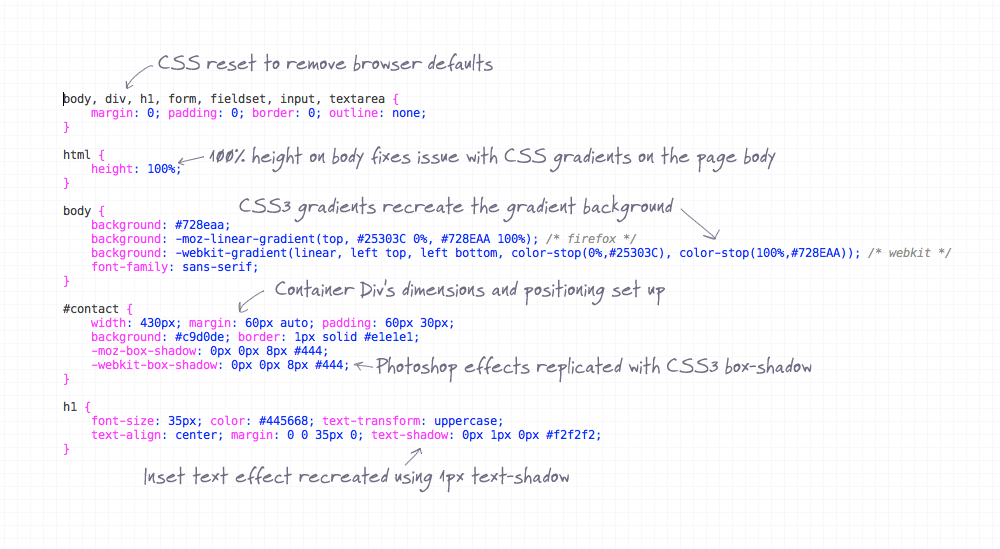
\includegraphics[scale=0.35]{img/css1.png}
 \end{center}
\end{frame}


\section{JavaScript / jQuery}

\section{JavaScript}

\begin{frame}
 \frametitle{JavaScript}
 JavaScript (JS) es un lenguaje de programación interpretado, Orientado a objetos, basado en prototipos, imperativo, débilmente tipado y dinámico.
 \newline
 Se utiliza principalmente en su forma del lado del cliente (client-side), implementado como parte de un navegador web permitiendo mejoras en la interfaz de usuario y páginas web dinámicas.
\end{frame}

\begin{frame}
 \frametitle{JavaScript}
 Al igual que con el código CSS, JavaScript se puede colocar en los sitios web ya sea incrustandolo en el código HTML, con la etiqueta script, o adjuntandolo en un archivo separado.
\end{frame}

\begin{frame}
 \frametitle{Estructura}
 \begin{center}
    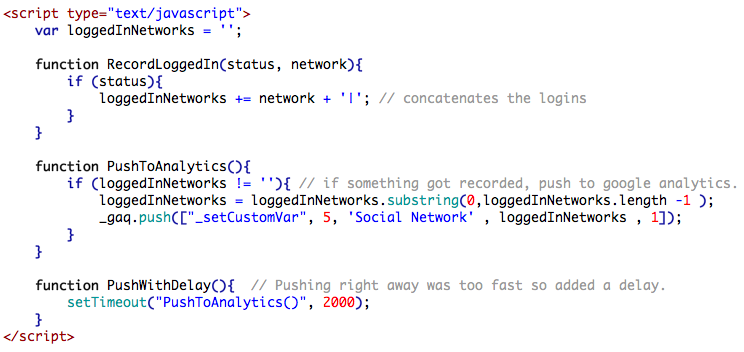
\includegraphics[scale=0.35]{img/js.png}
 \end{center}
\end{frame}


\section{PHP}

\section{SQL / PostgreSQL}

\section{Laravel}

\section{TODO}

\frame{
  \vspace{2cm}
  {\huge ¿ Preguntas ?}

  \vspace{3cm}
  \begin{flushright}
    Sebastián Salazar Molina

    \structure{\footnotesize{sebasalazar@gmail.com}}
  \end{flushright}
}

\end{document}
